\documentclass[border=10pt]{standalone}
\usepackage{tikz,amsmath}
\usetikzlibrary{arrows.meta}

% ========== 配色 ==========
\definecolor{inFill}{RGB}{183,224,177}
\definecolor{inLine}{RGB}{32,102,32}
\definecolor{hidFill}{RGB}{199,203,243}
\definecolor{hidLine}{RGB}{52,58,143}
\definecolor{orFill}{RGB}{250,224,180}
\definecolor{orLine}{RGB}{190,110,20}
\definecolor{outFill}{RGB}{243,199,199}
\definecolor{outLine}{RGB}{143,52,52}
\definecolor{blFill}{RGB}{214,228,250}
\definecolor{blLine}{RGB}{60,90,170}

\begin{document}
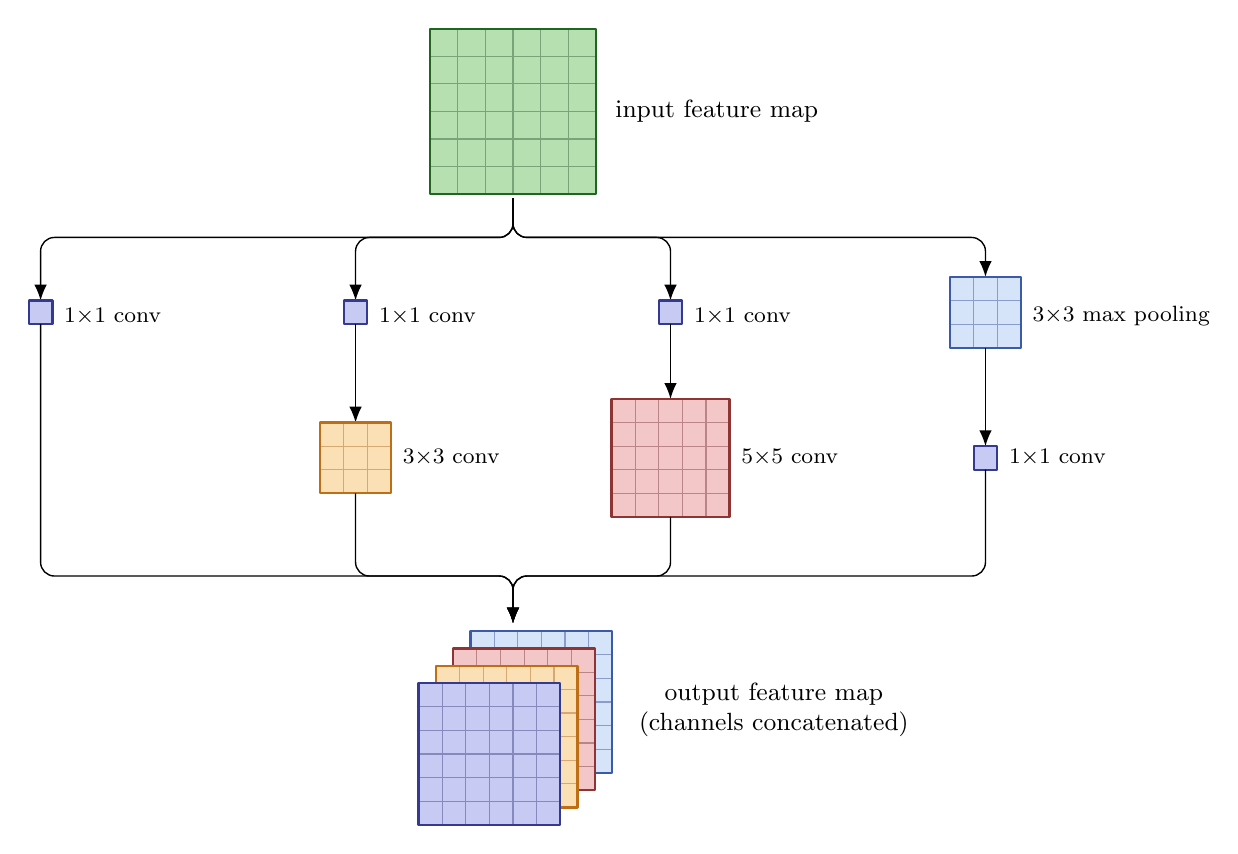
\begin{tikzpicture}[
    font=\small, line join=round,
    every node/.style={inner sep=0pt, outer sep=0pt},
    >={Latex[length=2mm, width=1.6mm]},
    arr/.style={->, line width=.5pt, rounded corners=5pt}
  ]

  % ========== 网格方块宏 ==========
  \newcommand{\gridbox}[5]{%
    \fill[#5Fill] (#1,#2) rectangle (#1+#3*#4, #2+#3*#4);
    \draw[step=#4, #5Line!60, line width=.4pt, shift={(#1,#2)}] (0,0) grid (#3*#4, #3*#4);
    \draw[#5Line, thick] (#1,#2) rectangle (#1+#3*#4, #2+#3*#4);
  }

  % ========== 顶部：输入特征图 ==========
  \gridbox{-1.05}{5.15}{6}{.35}{in}
  \node[anchor=west] at (1.3,6.2) {input feature map};

  % ========== 输入 -> 四分支（接到第一级盒顶） ==========
  \draw[arr] (0,5.1) -- (0,4.6) -- (-6,4.6) -- (-6,3.8);
  \draw[arr] (0,5.1) -- (0,4.6) -- (-2,4.6) -- (-2,3.8);
  \draw[arr] (0,5.1) -- (0,4.6) -- (2,4.6)  -- (2,3.8);
  \draw[arr] (0,5.1) -- (0,4.6) -- (6,4.6)  -- (6,4.1);

  % ========== 第一级：1x1=1格；3x3 pool=3x3格（中心 y=3.2） ==========
  \gridbox{-6.15}{3.5}{1}{.3}{hid}
  \node[anchor=west, font=\footnotesize] at (-5.7,3.6) {1$\times$1 conv};
  \gridbox{-2.15}{3.5}{1}{.3}{hid}
  \node[anchor=west, font=\footnotesize] at (-1.7,3.6) {1$\times$1 conv};
  \gridbox{1.85}{3.5}{1}{.3}{hid}
  \node[anchor=west, font=\footnotesize] at (2.3,3.6) {1$\times$1 conv};
  \gridbox{5.55}{3.2}{3}{.3}{bl}
  \node[anchor=west, font=\footnotesize] at (6.6,3.6) {3$\times$3 max pooling};

  % ========== 第一级 -> 第二级（盒底 -> 盒顶） ==========
  \draw[arr] (-2,3.5) -- (-2,2.25);
  \draw[arr] (2,3.5)  -- (2,2.55);
  \draw[arr] (6,3.2)  -- (6,1.95);

  % ========== 第二级：3x3=3x3格；5x5=5x5格；1x1=1格（中心 y=0.8） ==========
  \gridbox{-2.45}{1.35}{3}{.3}{or}
  \node[anchor=west, font=\footnotesize] at (-1.4,1.8) {3$\times$3 conv};
  \gridbox{1.25}{1.05}{5}{.3}{out}
  \node[anchor=west, font=\footnotesize] at (2.9,1.8) {5$\times$5 conv};
  \gridbox{5.85}{1.65}{1}{.3}{hid}
  \node[anchor=west, font=\footnotesize] at (6.3,1.8) {1$\times$1 conv};

  % ========== 四分支 -> 汇合 -> 拼接堆（从第二级/第一级盒底出发） ==========
  \draw[arr] (-6,3.5) -- (-6,0.3) -- (0,0.3) -- (0,-0.3);
  \draw[arr] (-2,1.35) -- (-2,0.3) -- (0,0.3) -- (0,-0.3);
  \draw[arr] (2,1.05)  -- (2,0.3)  -- (0,0.3) -- (0,-0.3);
  \draw[arr] (6,1.65)  -- (6,0.3)  -- (0,0.3) -- (0,-0.3);

  % ========== 底部：通道维拼接 ==========
  \gridbox{-0.54}{-2.2}{6}{.3}{bl}
  \gridbox{-0.76}{-2.42}{6}{.3}{out}
  \gridbox{-0.98}{-2.64}{6}{.3}{or}
  \gridbox{-1.2}{-2.86}{6}{.3}{hid}
  \node[anchor=west, align=center] at (1.6,-1.4)
    {output feature map\\(channels concatenated)};

\end{tikzpicture}
\end{document}